\chapter{基于深度学习的自动驾驶系统蜕变测试框架}

\section{引言}

上一章中提到了DeepTest设计了一个试图模拟现实世界驾驶场景的图像,进而自动生成测试用例的测试系统,但它合成图像的主要方式是在原驾驶图像上应用仿射变换,添加各种效果图层,比如雾天、雨天和模糊效果
,然后检测自动驾驶系统在原图和合成图上的输出行为是否一致。通过大量的原始和合成后的驾驶场景图,DeepTest以一种相对快速和廉价的方式成功地在一些开源的自动驾驶模型中检测出了各种不一致的驾驶行为。

\begin{figure}[h]
    \centering
    \subfigure[DeepTest]{
        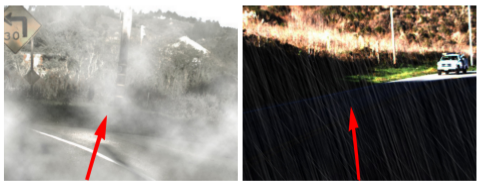
\includegraphics[width = 0.7\textwidth]{deeptest_effect}
    }
    \subfigure[DeepRoad]{
        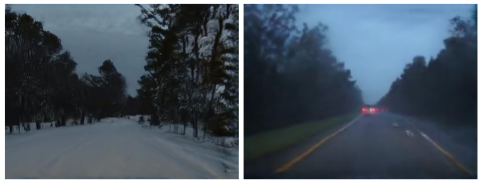
\includegraphics[width = 0.7\textwidth]{deeproad_effect}
    }
    \caption{天气场景合成效果图比较}
    \label{label-deep}
\end{figure}

但是我们认为DeepTest用于合成测试用例的方法并不能真实地反应出现实中的驾驶场景。比如现实中由车载摄像头拍摄的驾驶场景很少会有仿射变换后的效果,通过应用在原图上的雾天、雨天和模糊效果来简单地模拟对应的天气场景下的图像也显得很不真实,这也降低了DeepTest检测结果的有效性和可靠性。比如
下图\ref{label-deep}a左图为DeepTest中添加的雾天效果,可以明显看出图中很多部分呈现出扭曲的状态,感觉就像是简单地调暗原图像素,然后加上简单的烟雾效果,事实上,我们简单地利用PhotoShop中的像素调节和图像叠加功能也合成了DeepTest中的图像。下图\ref{label-deep}a右图则显示了DeepTest使用的雨天效果变换,类似地,DeepTest也是通过简单地将许多白色线条加到了原图上来模拟雨天场景的。这样合成的雨天场景图片相比前者更加的不真实,因为在现实的雨天场景中,摄像头上往往会有雨滴,从而呈现出模糊的效果。DeepTest中只有极少的合成图像跟真实的驾驶场景类似,使得我们很难判断利用DeepTest检测出的错误驾驶行为到底是由原本基于深度神经网络的自动驾驶系统的缺陷导致,还是由于DeepTest本身的测试技术的不足导致的。除此之外,还有许多各种可能的真实驾驶场景是不能通过简单的图像变换技术来合成模拟的。比如大学天气下的道路场景,对于道路和合成渲染过程需要多种复杂的变换同时应用到原图上,道路旁边的物体,比如树木也是如此。

为了沿用DeepTest测试的核心思想,自动地为自动驾驶系统合成大量的真实驾驶场景的图像,我们参考DeepRoad测试技术设计了一个无监督测试框架。利用深度学习中的对抗生成网络技术来合成一些很难由人工采集到的各种天气场景下的路况图像。除此之外,我们基于DeepTest的工作,设计了一套针对基于深度神经网络自动驾驶系统的一个蜕变测试模块,核心思想为:无论真实的驾驶场景图像对于各种天气场景被以何种方式合成,自动驾驶系统对于原图和合成图做出的驾驶行为输出我们期望始终保持一致。基于此点,DeepRoad使我们能够测试基于深度神经网络的自动驾驶系统在各种天气场景下的精确性和可靠性,合成的各种极端天气场景下的图像集,比如大雪大雨天气的场景图像也能够扩充自动驾驶系统原有的数据集测试用例覆盖率,从而有助于提高自动驾驶系统的稳定性和鲁棒性。图\ref{label-deep}b为DeepRoad合成的雪天和雨天的驾驶场景图像,已经很难从真实的图像中区分,并且通过简单的图像转换技术很难合成类似的效果。

虽然DeepRoad可以用来合成各种天气场景的驾驶图像,在我们实验过程中,我们主要针对雪天和雨天场景进行了驾驶场景图像的合成工作。基于对抗生成网络技术,我们利用网络爬虫技术Scrapy从Youtube视频网站上收集了2组极端天气场景下的驾驶图像集,将真实的驾驶场景图像转换到对应的天气场景下的驾驶场景。此外,我们将合成的图像用于测试Udacity开源的自动驾驶系统\cite{udacity_as},实验结果显示DeepRoad检测出了上千种这些系统不同级别的行为不一致现象,表明自动驾驶系统的测试工作还有很大的提升空间。

\section{方法}

\subsection{深度神经网络蜕变测试}

蜕变测试在传统软件测试方法里被广泛应用于测试用例的自动生成以及BUG检测,蜕变测试的强大之处主要在于它能通过各种蜕变关系解决传统测试的Oracle问题。令$p$为程序的数学表示形式:一个将程序输入映射到程序输出的函数,即$p(i) = o$,同样地,令函数$f_I$和$f_O$分别表示程序输出集合输出集的映射函数,则一个蜕变关系可表示为:
\begin{gather}
    \centering
    \forall i, p(f_I(i))=f_O(p(i))
    \label{f:mt}
\end{gather}
基于这样的蜕变关系,令$\hat{p}$表示程序$p$的一个具体实现,则我们可以通过检测公式$\hat{p}(f_I(i))=f_O(\hat{p}(i))$是否对任意输入$i$都成立来测试程序$\hat{p}$的鲁棒性。通过利用蜕变关系交叉检验程序输入输出,从而测试程序具体实现的方法称为蜕变测试。例如给定一个实现$sin$函数的程序,我们可以利用蜕变测试来构造各类新的测试用例,而不用担心测试的对照物,即测试Oracle问题。对任意用于测试$sin$函数的输入$i$,有许多客观事实可以用于该测试的蜕变关系,比如$sin(-i)=sin(i)$以及$sin(i+2\pi)=sin(i)$。特别的对于这里蜕变关系的第一个例子有:$f_I(i)=-f_O(i)=-i$,对于第二个例子则是$f_I(i)=f_O(i)=i$。利用这样的蜕变关系,我们能够将已有的测试用例通过$f_I$生成一些新的测试用例,然后基于$f_O$来检验程序的输出。

在本工作中,我们进一步地将蜕变测试应用到了基于深度神经网络自动驾驶系统的测试当中。正式地,令$DNN$表示将每张路况图像映射到预测的方向盘拐角信号的基于深度神经网络的自动驾驶系统,给定原始图像集$\mathbb{I}$,定义各种图像变换$\mathbb{T}$,变换可以改变图像的路况场景,而不影响每张图像$i\in \mathbb{I}$的预测结果(即预测的拐角对于雨天和雪天场景下相同的路况图片应该几乎一致)。通过这样的方式,对于利用各类额外的变换图像输入来测试自动驾驶系统,我们可以得到下面的蜕变测试:
\begin{gather}
    \forall i \in \mathbb{I} \wedge \tau \in \mathbb{T}. DNN[\tau(i)]=DNN(i)
\end{gather}

\subsection{基于深度神经网络的路况图像变换}

关于自动驾驶系统测试的最新工作DeepTest\cite{DeepTest}也将蜕变测试用在了基于深度神经网络的自动驾驶系统测试中,但它只作了一些简单的图像合成转换,例如添加雾天、雨天和雪天的图层,因此导致有以下问题的存在:1). DeepTest可能会产生不真实的测试用例;2). DeepTest不能模拟复杂的道路场景变换(比如雪天场景)。

为了完善DeepTest工作,全自动地产生各种真实场景下的路况图像,我们利用UNIT\cite{UNIT},一个基于深度神经网络的方法来进行无监督图像到图像的变换。UNIT的核心思想是不同图像集的一组图像可以被映射到一个共享潜在空间,并有相同潜在表征。通过这样映射的方式,可以将来自某个图像集的图像(比如原始的路况图像),UNIT可以自动地合成另对应于另一个图像集(比如雨天的路况图像集)的图像,具体实现上,UNIT由对抗生成网络变分自编码器构成。

\begin{figure}[h]
    \centering
    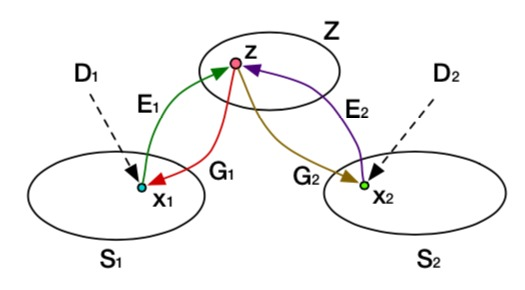
\includegraphics[width=.7\textwidth]{UNIT}
    \caption{UNIT模型结构}
    \label{unit-struct}
\end{figure}

图\ref{unit-struct}描述了UNIT模型的基本架构,其中$S_1$和$S_2$记为两组不同的图像集,$E_1$和$E_2$为2个将图像集分别从$S_1$和$S_2$投射到共享隐空间$Z$的自编码器。令$x_1$和$x_2$为共享同内容信息的对应图像,理想情况下$E_1$和$E_2$能将他们编码到相同的隐向量$z$。$G_1$和$G_2$为2个不同图像域的生成器,可将隐向量分别映射回$S_1$和$S_2$图像集中。$D_1$和$D_2$是两个判别器,可以检测出图像属于$S_1$还是$S_2$。理想情况下,判别器不能区分输入图像是来自目标图像域还是训练好的生成器。基于上述的自编码器和生成器,UNIT可以用来在两个不同图像域中转换图像,比如图像$x_1$可以通过$G_2(E_1(x_1))$转换到图像集$S_2$中。

UNIT的学习目标可以分解为优化以下3个损失函数:
\begin{itemize}
    \item \textbf{变分自编码器损失函数} 对每组编码器和生成器$<E_i,G_i>$最小化图像的重构损失。
    \item \textbf{对抗生成网络损失函数} 在对抗器和判别器对$<G_i,D_i>$的最小最大函数中找到最优值,使得$D_i$不能区分图像$x_i$是来自原图像集$S_i$还是生成器$G_i$。
    \item \textbf{循环一致损失函数} 对每组$<E_i,G_j,E_j,G_i>$最小化他们的循环重构损失,理想情况下有$x_1=G_1(E_2(G_2(E_1(x_1))))$以及$x_2=G_2(E_1(G_1(E_2(x_2))))$
\end{itemize}

总的损失函数可归纳为以下:
\begin{equation}
\begin{aligned}
    \min_{E_1,E_2,G_1,G_2}\max_{D_1,D_2}\mathb{L}_{CC_1}(E_1,G_2,E_2,G_1)+ \\ 
    \mathb{L}_{CC_2}(E_2,G_1,E_1,G_2) + \mathb{L}_{VAE_1}(E_1,G_1)+\mathb{L}_{VAE_2}(E_2,G_2)+ \\
    \mathb{L}_{GAN_1}(D_1,G_1) + \mathb{L}_{GAN_2}(D_2,G_2)
    \label{f:unit}
\end{aligned}
\end{equation}

\subsection{测试框架整体架构}

\begin{figure}[h]
    \centering
    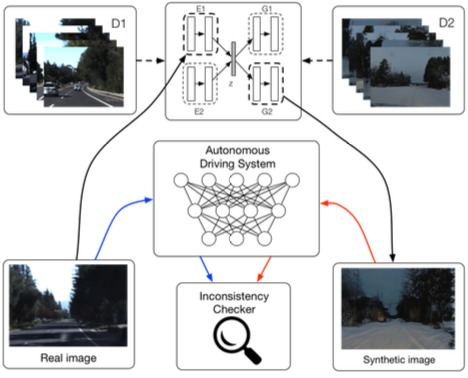
\includegraphics[width=.7\textwidth]{deeproad_wf}
    \caption{DeepRoad架构}
    \label{dp-wf}
\end{figure}

上图\ref{dp-wf}为我们为基于深度神经网络自动驾驶系统设计的蜕变测试框架。如图所示,DeepRoad首先从目标图像集(即一组晴天路况图像集和一组雨天路跨那个图像集)选出一组无配对的训练图集,然后利用无监督框架UNIT将这两组图像集利用公式\ref{f:unit}中的损失函数,映射到同样的隐空间。我们从Udacity开源的真实路况数据集\cite{udacity_dataset}采样了晴天路况图,从Youtube视频收集了雪天和雨天的路况图集,然后将他们作为UNIT的训练集进行模型的训练。模型训练完成后,DeepRoad再利用成型的UNIT将整个Udacity图像集转换成另一个场景的路况图像集(雪天场景或者雨天场景)。即给定任一原始的晴天驾驶场景图像$i$,DeepRoad可以利用训练好的UNIT模型合成出原始图像在另一个天气场景下对应的图像(即雨天场景),记为$\tau(i)$。最后DeepRoad将每组配对的真实图像和合成图像送入自动驾驶系统进行测试,即检测$DNN[\tau(i)]=DNN[i]$是否成立,从而检测自动驾驶系统的不一致输出行为。因为路况合成图像对驾驶行为,即方向盘拐角,不会有较大影响,因而任一不一致的输出都可能反应了自动驾驶系统在测试框架下显示出的鲁棒性问题。

\section{实验}

\subsection{实验数据和数据预处理}

我们使用由Udacity提供的真实数据集作为检验自动驾驶系统不一致行为的基准数据,从该数据集中选取了2段高速公路驾驶视频,视频中道路的光线和路况随着时间变化有明显的改变。为了训练相应的UNIT模型,我们也从Youtube上收集了各种极端场景下的路况图像。具体实验阶段,我们选择了雪天和大雨天气下的路况图像来转化真实场景的驾驶路况图像。为了扩充收集到图像集的多样性,我们只搜索了时长超过20分钟的视频。在大雨场景的视频里,通常会有雨刷扫过车窗的情形,这对图像数据而言是噪声数据,因此在数据的预处理阶段,我们人工的检查和筛除了有雨刷出现的图像。除此之外,实验中所有使用的图像在实验之前都被裁剪成$240\times 320$的大小,并且对从Youtube上收集的视频进行了低频采样,以避免有过于相近的连续图像帧出现在最终的数据集里。

\subsection{自动驾驶系统模型}

我们基于Udacity开源的3个深度神经网络自动驾驶系统模型对我们的测试框架进行评估,分别有:Autumn\cite{autumn},Chauffeur\cite{Chauffeur}和Rwightman\cite{Rwightman}。我们使用这3个模型作是因为他们都是预训练好的模型,且可以直接在合成数据集上进行驾驶拐角预测。其中Rwightman模型的实现细节没有公开,但是基于黑盒测试原理,我们的方法目的是检测模型输出的不一致行为而不是定位软件的错误,因此我们仍然使用Rwightman作为我们的评价模型。

\textbf{Autumn}. Autumn由一个数据预处理模块和一个卷积神经网络构成。具体实现上,Autumn首先计算输入图像的光线流,然后将他们输入到卷积神经网络中预测方向盘拐角。Autumn的网络结构为:3层步长为2的$5\times 5$的卷积层,2层$3\times 3$的卷积层加上5个全连接层。模型由OpenCV,Tensorflow和Keras框架实现。
\textbf{Chauffeur}. Chauffeur由一个卷积神经网络和一个有LSTM单元递归神经网络(RNN)构成。工作流程为:卷积神经网络首先提取输入图像的特征,然后利用RNN对之前的100张连续图像进行方向盘拐角预测。该模型也是通过Tensorflow和Keras实现的。

\subsection{评价指标}

基于我们的假设,如果方向盘拐角的预测值在修改了路况图像的天气场景后不发生改变的话则被测试的自动驾驶系统可被视为是稳定的。但是这个假设条件太苛刻了,因为由于图像场景改变导致的微小的拐角差也可以落在安全的拐角区域。因此,我们放宽了之前的假设条件,如果原图和合成图的预测拐角差值能够在一定的误差范围内,我们也接受该预测拐角值。我们将被测试的自动驾驶系统中出现的不一致预测行为次数定义为:
\begin{gather}
    IB(DNN,\mathbb{I})=\sum_{i\in \mathbb{I}}f(|DNN[i]-DNN[\tau(i)]|>\epsilon)
\end{gather}
这里的$DNN$记为自动驾驶系统模型,$\mathbb{I}$为真实场景的驾驶图像数据集,$i$为图像集$\mathbb{I}$中第$i$张图像。$\tau$记为能够实现输入图像天气场景转换的图像生成器。函数$f$为输出为1或0的指示函数,$\epsilon$为允许的误差范围。

\subsection{实验结果}

\begin{figure}[htb]
    \centering
    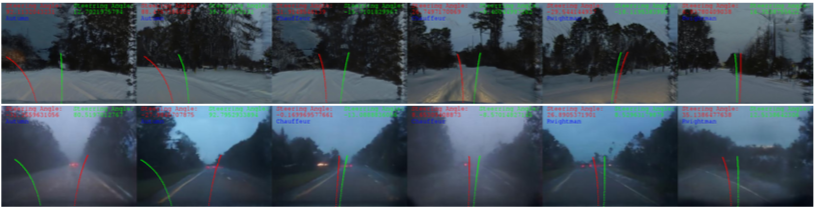
\includegraphics[width=\textwidth]{inconsist}
    \caption{自动驾驶系统在真实图和合成图上表现的不一致行为}
    \label{inconsist}
\end{figure}

图\ref{inconsist}为检测到自动驾驶系统不一致行为的样例图,第一行为雪天场景的图,第二行为雨天场景的图。每张小图中,蓝色的字为模型的名称,红色和绿色的字为真实图和合成图的预测拐角值。图中的曲线描述了预测值即方向盘拐角,帮助我们检验差值。从图中我们可以观察到模型Autumn模型中出现的不一致行为数最多,反之,模型Rwightman相对而言是最稳定的自动驾驶系统模型。图\ref{inconsist}也表明DeepRoad能够在不同天气场景下对真实的自动驾驶系统发现各种不一致行为。比如像Autumn和Chauffer的自动驾驶系统模型(在Udacity的自动驾驶系统竞赛中它们是排名最高的2个算法),在晴天的驾驶场景下表现相当出色,但在雨天或雪天的场景下可能会撞向路边或是其他的车辆。

\begin{figure}[]
    \centering
    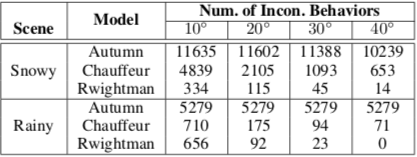
\includegraphics[width=.5\textwidth]{inconsist-t}
    \caption{不同天气场景及误差限下检测到的不一致行为数}
    \label{inconsist-t}
\end{figure}

图\ref{inconsist-t}展示了在不同天气场景、不同的误差界限下对各个自动驾驶系统模型检测到的不一致行为的具体数量。比如当检测的场景为雨天,误差限设为$10\degree$时,DeepRoad对3中自动驾驶系统分别检测到了5279,710和656种不一致行为。从表中我们也观察到Autumn在两种天气场景下检测到的不一致行为数目是最多的。我们认为一个可能的原因是因为Autumn是完全基于基于卷积神经网络的结构,不能像反馈神经网络一样利用到前验历史信息,因而导致系统不能在所有的驾驶场景下都能表现出很好的鲁棒性。另一方面,Rwightman比其他两个模型在雨天和雪天场景,以及各个误差限下都表现出更好的驾驶行为一致性。以上表明DeepRoad不仅能检测出自动驾驶系统上千种不一致的驾驶行为,还能就每个自动驾驶系统的鲁邦性作出评估,比如仅靠Udacity原始的数据集,很难发现类似Autumn这样的自动驾驶系统在雨天和雪天场景下的局限性。

\section{本章小结}

我们介绍了一个基于DeepRoad\cite{DeepRoad},利用无监督对抗生成网络的技术来测试深度神经网络自动驾驶系统的蜕变测试框架。它使用蜕变测试技术检测自动驾驶系统在不同的天气场景下所表现出不一致的驾驶行为。除此外,实验结果表明该测试框架在检测自动驾驶系统鲁邦性上也有很好的应用价值。目前它只支持两种天气场景下的测试用例转换,在后面的章节将介绍我们针对提高自动生成的测试用例质量,即驾驶场景图像的合成质量,以及驾驶场景的种类扩充所做的后续工作。